\chapter{Decoration}
Decoration is a very big field, which deserves a separate book to cover it in 
detail. Here we will only discuss some of the main techniques for using glazes 
and engobes.
%-------------------------------------------------------------------------------
\section{Decoration and Design}
The main reason for decorating pots is for pure enjoyment. As pottery is 
something that is used intimately every day, it should be attractive and 
interesting, besides being simply functional. Decorated pottery also has a 
better market value and often more than pays for the extra time taken.
Good decoration is always related to the design of the pot. It should be used 
to emphasize and enhance the shape of the pot, rather than being applied 
randomly.

There are several approaches to decoration:
%-------------------------------------------------------------------------------
\subsubsection{Banding}
Plain or decorative bands of color are painted around the pot, usually by 
spinning the pot on a banding wheel and applying color with a brush. The bands 
are placed where they emphasize changes in the curve of the pot, for example, 
at the rim, the belly, the shoulder.
%-------------------------------------------------------------------------------
\subsubsection{Area Decoration}
Decoration is placed inside a defined area, such as a circle. Again this should 
be done to emphasize the natural curves of the pot.
%-------------------------------------------------------------------------------
\subsubsection{Overall Patterns}
These are patterns that are repeated around the pot, often expanding and 
contracting as the pot does.
%-------------------------------------------------------------------------------
\subsubsection{Contrasting Shapes}
These are strongly shaped areas of pattern or color that contrast with the 
shape of the pot.
%-------------------------------------------------------------------------------
\subsection{Motifs, Styles, Local Inputs}
There are as many motifs and styles of decoration as there are cultures in the 
world. In traditional cultures, motifs are selected from mythology and familiar 
designs. Nowadays, with the mixing of cultures around the world, pots are often 
designed for what can be marketed for export, and design tends to be based on 
fashion rather than tradition.

The potter selling to tourists will generally choose traditional motifs, since 
tourists are interested in the culture of the area.
%-------------------------------------------------------------------------------
\section{Glaze Decoration}
Glaze decoration is done with the glaze itself or with colorants under the 
glaze or on top of the glaze.
%-------------------------------------------------------------------------------
\subsection{Underglaze}
Underglaze decoration is decoration that is applied under the glaze. It is 
affected by the transparency and fluidity of the glaze.

Underglazing is usually done under a transparent glaze in order to show it 
clearly. However, beautiful effects can be obtained under opaque or semiopaque 
glazes.

A variety of pigments and oxides may be used.
%-------------------------------------------------------------------------------
\subsubsection{Metallic Oxides}
The more fusible metallic oxides can be used directly as underglaze pigments, 
mixed thinly with water. The satisfactory ones are red iron oxide, cobalt 
carbonate, manganese dioxide and copper carbonate. Designs made with oxides 
alone will often run with the glaze. Refractory oxides, such as chrome oxide 
and rutile, can cause crawling.
%-------------------------------------------------------------------------------
\subsubsection{Oxides Mixed With Glaze}
Metallic oxides can be mixed about 50/50 with glaze, which will prevent the 
problem of crawling. However, the decoration will usually flow with the glaze 
and should be designed with this in mind.
%-------------------------------------------------------------------------------
\subsubsection{Underglaze Pigments}
These are pigments that are specially prepared by fritting metallic oxides in a 
base glaze that fires hard but is not fluid. Rather than preparing them 
yourself, it is usually better to purchase commercial underglazes from a 
supplier. These are supplied for venous firing temperatures and firing 
conditions in a wide range of colors. Not all colors can be used under all 
conditions, and suppliers can usually tell you which are suitable for oxidation 
and reduction and what type of base glaze will develop the best colors.
%-------------------------------------------------------------------------------
\subsection{On-Glaze}
On-glaze decoration is applied on top of the unfired glaze. It may be done with 
a contrasting color of glaze or with metallic oxides or glaze pigments.

Application is done by brushing or spraying. Even more than underglaze, 
on-glaze decoration will tend to flow with the glaze. If distinct patterns are 
desired, a stiff, viscous glaze will give the best results.
%-------------------------------------------------------------------------------
\subsubsection{Double Glazing}
Glazes high in surface tension (see section~\ref{sec:surfacetension}) tend to 
form into small islands on melting. This may cause crawling, but it can also be 
used as a decorative effect by applying two different glazes on top of each 
other. The glazes must have different degrees of surface tension. This is 
achieved by adding clay or talc to one of the glazes. The colors should be 
contrasting. The best results are obtained with a light-colored glaze at the 
bottom.
%-------------------------------------------------------------------------------
\begin{figure}[htbp!]
  \centering
  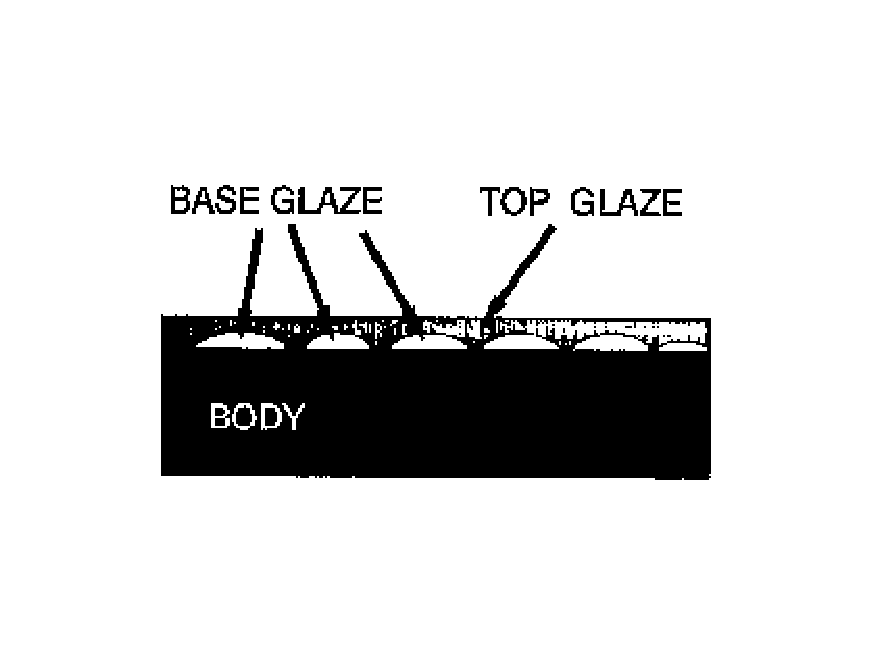
\includegraphics[width=0.7\linewidth]{img/doubleglazinghigh.eps}
  \caption{Double glazing with the high-surface-tension glaze on top. This 
  draws itself into islands leaving the bottom glaze in irregular patterns.}
  \label{fig:doubleglazinghigh}
\end{figure}
%-------------------------------------------------------------------------------
\begin{figure}[htbp!]
  \centering
  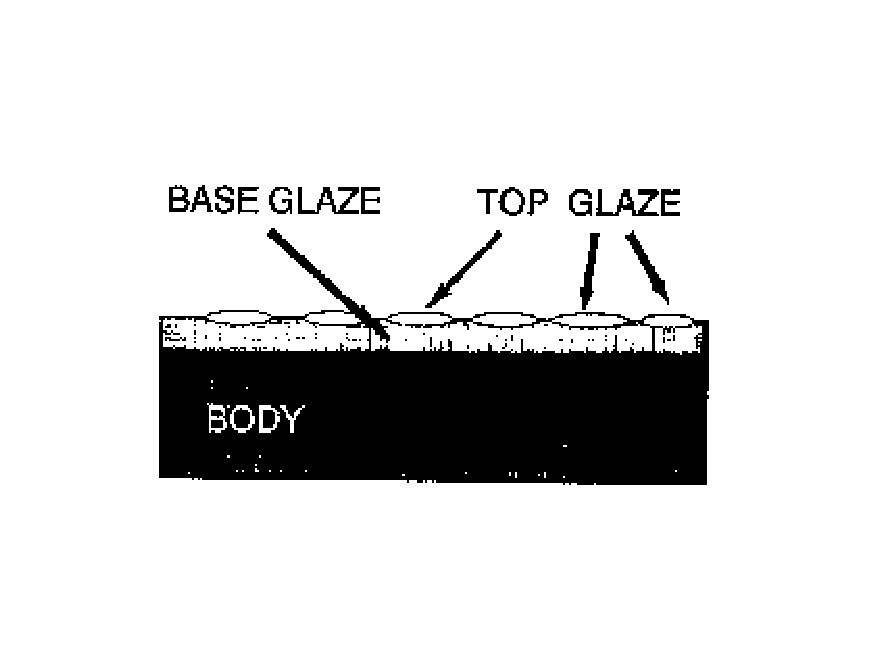
\includegraphics[width=0.7\linewidth]{img/doubleglazinglow.eps}
  \caption{Double glazing with the low-surface-tension glaze on top. This 
  produces a different effect.}
  \label{fig:doubleglazinglow}
\end{figure}
%-------------------------------------------------------------------------------
\subsection{Overglaze}
Overglaze decoration is often called ``china painting''. The pot is glaze-fired 
as usual and then is decorated with special low-temperature enamels that fire 
at around 700\degree C. The enamels are prepared from color pigments and 
low-temperature frits and are best purchased from commercial suppliers. They 
are available in every color and have the advantage of firing to true colors, 
making them suitable for elaborate painting effects. They also stay where they 
are applied, as there is no chance of the glaze running at this low temperature.

Overglaze is available as powder, which must be mixed with a medium. This is 
best done by grinding the pigment and medium on a glass plate with a thin 
palette knife.

Sometimes plain water is used: this works well when filling areas with solid 
colors. It helps to add some water-soluble glue (white glue) to provide dry 
strength.

For more elaborate painting, pigment is mixed with special oils. The best is 
oil of lavender, which is thickened as desired with a thicker oil. The 
consistency is controlled very much like with oil paint.

Some suppliers have ready-mixed overglaze, which comes in tubes. This can be 
used directly, without grinding.

Special metallic or iridescent overglazes are known as ``luster''. These are 
available commercially as liquid gold, platinum and a variety of mother of 
pearl colors. They also are fired at 700\degree C. 

\textbf{Note:} Lusters take on the same surface as the glaze, i.e. a matt glaze 
will produce a matt luster and a shiny glaze will give a mirror-like effect.

Overglazes are applied by brushing or by spraying.
%-------------------------------------------------------------------------------
\subsubsection{Overglaze Transfers or Decals}
Most commercially sold decorated dinnerware is decorated with decals (sometimes 
called transfers), which are made from overglaze that is silkscreen-printed 
onto decal paper. These are available from suppliers in a range of standard 
designs and can also be custom-made (in large quantities). They are applied to 
already glaze-fired ware.

The decal is soaked in water until the design can easily be slid off the paper. 
The wet paper is placed in the correct location and is carefully slid from 
under the design, leaving the design adhered to the pot. The design is 
carefully smoothed, dried and fired like standard overglaze.
%-------------------------------------------------------------------------------
\subsection{Reglazing, Multiple Glazing}
Reglazing means applying glaze and firing an article that already has been 
fired once. It is sometimes necessary when glazes do not work correctly the 
first time -they may be too thin, underfired or not the right color.

Multiple glazing is the process of glazing and firing an article two or more 
times in order to get special glaze effects that cannot be achieved in one 
firing. It often involves first glaze firing the pot at a high temperature and 
then glaze firing with lower temperature glazes, in order to get special colors 
or textures. For example, a pot may be fired to cone 10, then be refired with 
cone 06 glazes to get bright colors. It may be fired several times at cone 010 
for overglazes and lusters.

Reglazing or multiple glazing makes an article more expensive, but it can also 
be sold at a much higher price.
%-------------------------------------------------------------------------------
\subsubsection{Reglazing Hints}

Because already fired ware is no longer porous, it is difficult to apply enough 
glaze. It helps to first heat the article (as hot as you can hold in your 
hand), and spraying is the most effective way to apply more glaze.

For multiple glazing, glaze can be specially prepared by adding cellulose gum 
(CMC). This thickens the glaze and gives it better handling strength.
%-------------------------------------------------------------------------------
\section{Engobe Decoration}
Engobe is a specialized type of clay slip that is used for decoration under the 
glaze. The engobe shows through a transparent or semitransparent glaze and can 
have the range of color that is possible in glaze.
%-------------------------------------------------------------------------------
\subsection{Advantages and Disadvantages, as Compared to Glaze Decoration}
Engobes stay where they are applied and do not run with the glaze. This makes 
it possible to do designs with sharp edges or a lot of detail.

Engobes are often used on dark clay bodies in order to provide a bright, white 
background for glazes.
%-------------------------------------------------------------------------------
\subsection{Engobe Making, Adjusting to Body}
Engobe is generally prepared as a white base and then colored with appropriate 
coloring oxides. If you are already using a white clay body, this becomes an 
engobe simply by thinning it with water. A dark body will require a white 
engobe formula that fits it correctly.

The main problem with engobe is getting a good fit between engobe and clay 
body. It must have about the same amount of shrinkage as the body or it will 
tend to flake off or crack. The engobe should also mature at the same 
temperature as the clay body in order to provide a strong clay-glaze interface. 

Usually engobes designed for plastic clay will not fit on bone dry or biscuit 
clay and vice versa.

Some typical engobe recipes are shown in table~\ref{tab:engoberecipes}

Engobes can be applied at three different stages.
%-------------------------------------------------------------------------------
\subsubsection{Leatherhard}
This is the best stage for applying engobes, as it permits the widest range of 
decorating techniques (brushing, incising, inlaying, stencil etc. -see below). 
The engobe must have enough clay in it to shrink at the same rate as the body.
%-------------------------------------------------------------------------------
\subsubsection{Bone-Dry}
Engobes for bone-dry application need to have less shrinkage, so that they 
adhere to the body.
%-------------------------------------------------------------------------------
\subsubsection{Biscuit}
Engobes for biscuit application are more like underfired glazes.
%-------------------------------------------------------------------------------
\begin{landscape}
\begin{center}
  \renewcommand{\arraystretch}{1.5}
  \begin{table}\centering
    \begin{tabular}{|c||c|c|c||c|c|c||c|c|c|}\hline
 \textbf{Temperature Range}
&\multicolumn{3}{c}{\textbf{Cone 08--1}}\vline
&\multicolumn{3}{c}{\textbf{Cone 1--6}}\vline
&\multicolumn{3}{c}{\textbf{Cone 6--11}}\vline\\\hline\hline
      
%-------------------------------------------------------------------------------
\textbf{Body Condition}
&\textbf{Damp}&\textbf{Dry}&\textbf{Biscuit}
&\textbf{Damp}&\textbf{Dry}&\textbf{Biscuit}
&\textbf{Damp}&\textbf{Dry}&\textbf{Biscuit}\\\hline\hline
%------------------------------------------------------------------------------
Kaolin&25&15&5&25&15&5&25&15&5\\\hline
%------------------------------------------------------------------------------
Ball Clay&25&15&15&25&15&15&25&15&15\\\hline
%------------------------------------------------------------------------------
Calcined Kaolin&-&20&20&-&20&20&-&20&20\\\hline
%------------------------------------------------------------------------------
Leadless Frit&15&15&15&-&-&5&-&-&5\\\hline
%------------------------------------------------------------------------------
Nepheline Syenite&-&-&-&15&15&20&-&-&5\\\hline
%------------------------------------------------------------------------------
Feldspar&-&-&-&-&-&-&20&20&20\\\hline
%------------------------------------------------------------------------------
Talc&5&5&15&5&5&5&-&-&-\\\hline
%------------------------------------------------------------------------------\\
Quartz&20&20&20&20&20&20&20&20&20\\\hline
%------------------------------------------------------------------------------
Opacifier (Zircon)&5&5&5&5&5&5&5&5&5\\\hline
%------------------------------------------------------------------------------
Borax&5&5&5&5&5&5&5&5&5\\\hline
%------------------------------------------------------------------------------
\end{tabular}
\caption{Typical Engobe Recipes per Daniel Rhodes.}
\label{tab:engoberecipes}
\end{table}
\end{center}
\end{landscape}
%-------------------------------------------------------------------------------
\subsubsection{Engobe Composition}
Engobe is made up of a mixture of plastic and nonplastic ingredients. Recipes 
for engobes look like those for glazes with a high percentage of refractory 
ingredients.

For white engobes, the plastic ingredients are china clay and ball clay. The 
amount of ball clay can be adjusted to get correct shrinkage.

The nonplastic ingredients are feldspar and quartz, and for low-temperature 
engobes frit is sometimes added to lower the vitrification point.

Small amounts of borax are often added to give better dry strength and to fuse 
the other ingredients together.

Engobes are often deflocculated like a casting slip, and in fact you can often 
use a casting slip which fires at the same temperature as your clay body.
%-------------------------------------------------------------------------------
\subsection{Color Oxide Additions to Engobe}
Coloring oxides are added to engobes as a percentage, as with glazes. However, 
since the color is diluted by the glaze over it, larger amounts are required. 
You should also remember that the oxide reactions will depend on the type of 
glaze being applied and on whether oxidation or reduction firing is used. 

As with glaze colorants, the most interesting colors are usually obtained by 
mixing combinations of oxides.

Table~\ref{tab:engobeoxides} shows the typical oxides used in engobes, and 
their resulting colors.
%-------------------------------------------------------------------------------
\begin{center}
  \begin{table}\centering
    \renewcommand{\arraystretch}{1.5}
\begin{tabular}{|c|c|c|}\hline
 \textbf{Oxide}&\textbf{Percent}&\textbf{Color}\\\hline\hline
&1--5\%&Light green to light brown\\\cline{2-3}
Red Iron Oxide&5--10\%&brown\\\cline{2-3}
&10--15\%&dark brown to black\\\hline
Copper oxide or carbonate&1--5\%&Green or blue. (Red in reduction)\\\hline
Cobalt oxide or carbonate&1--5\%&Light to dark blue\\\hline
Chrome oxide&1--5\%&Green\\\hline
Manganese oxide&1--10\%&Purple-brown\\\hline
Nickel oxide&1--5\%&Grey or green-grey\\\hline
Titanium dioxide (Rutile)&1--10\%&Tan, or mottled colors\\\hline
Commercial stains&1--50\%&The color of the stain\\\hline
\end{tabular}
\caption{Typical oxide amounts in engobes, and the resulting colors.}
\label{tab:engobeoxides}
\end{table}
\end{center}
%-------------------------------------------------------------------------------
\subsection{Application Methods}
A wide variety of decoration techniques can be used with engobe. Leather-hard 
ware permits the largest variety of techniques and usually has fewer technical 
problems compared to application on bone-dry or biscuit ware. Work flow for 
leather-hard engobe decoration is:
%-------------------------------------------------------------------------------
\begin{enumerate}
  \item Apply the engobe
  \item Biscuit fire
  \item Apply the glaze
  \item Glaze fire
\end{enumerate}
%-------------------------------------------------------------------------------
\subsubsection{Dipping, Pouring}
This is done the same as with glazes. The engobe should be just thick enough to 
completely cover the clay. Too thick application will often crack, especially 
on rims. If applied leather-hard, pouring and dipping should be done quickly, 
so that the pot does not get too soft from absorbing water.
%-------------------------------------------------------------------------------
\subsubsection{Brushing}
Brushing is one of the most satisfactory methods, especially for making bands 
or areas of engobe. The technique requires some skill in order to get an even 
coating. The brush should be fully loaded with engobe and should spread it 
evenly.
%-------------------------------------------------------------------------------
\subsubsection{Spraying}
The engobe must be thin enough to flow through the spray gun. It should be 
applied in several even coats, taking care to keep a smooth surface and to 
cover all areas equally.
%-------------------------------------------------------------------------------
\subsubsection{Scratching or ``Sgraffito''}
To get fine lines, engobe is applied to an area and, after it sets, it is 
scratched with a sharp tool. This is called ``sgraffito'', which means 
``scratching''. The clay color shows as a line.
%-------------------------------------------------------------------------------
\subsubsection{Inlay}
Lines are scratched on the leather-hard pot and then filled with engobe. The 
excess engobe is removed with a metal scraper after it sets, or with sandpaper 
after the pot is bone-dry. This results in a smooth surface, with the engobe 
lines contrasting with the clay colon
%-------------------------------------------------------------------------------
\subsubsection{Stencil}
Paper or plastic stencils are placed on the leather-hard pot, and engobe is 
brushed or sprayed over them. Afterwards the stencil is removed leaving the 
design of the stencil.
%-------------------------------------------------------------------------------
\subsubsection{Trailing}
Usually called ``slip'' trailing, the engobe is applied by allowing it to flow 
from a device with a small opening, which produces raised line decoration. It 
is easiest to use a rubber bulb (such as an ear syringe available in 
pharmacies) or plastic containers used for soap or cosmetics. The opening can 
be made smaller by inserting small metal tubes.
%-------------------------------------------------------------------------------
\subsubsection{Hints}
Engobes will show most clearly under a fully transparent glaze. However, 
semitransparent or even opaque glazes can give beautiful effects, clouding the 
engobe colors.

Sophisticated decorators can take advantage of different glazes over the engobe 
to produce different colors. Complicated effects can result from applying 
different glazes to different areas of the decorated piece.
%-------------------------------------------------------------------------------
\subsection{Engobe Problems}
Often engobe will come off the pot. This almost always is caused by a different 
shrinkage rate of clay body and engobe and usually happens before firing. In 
many cases the engobe is applied too thick.
%-------------------------------------------------------------------------------
\subsubsection{Engobe Shrinks More Than The Clay Body}
In this case, the engobe will develop cracks and will flake off, with the 
flakes curling away from the ware. The solution is to reduce the amount of 
plastic clay or substitute raw clay with calcined clay. Deflocculating usually 
helps.
%-------------------------------------------------------------------------------
\subsubsection{Engobe Shrinks Less Thank The Clay Body}
In this case, the engobe will flake off, especially on rims and sharp edges, 
and the flakes will be flat. The solution is to add more plastic clay or to 
substitute calcined clay with raw clay.
%-------------------------------------------------------------------------------
\subsubsection{Flaking After Firing}
This is caused by differences in firing shrinkage between clay and engobe. 
Usually adding flux to the engobe will help.
%-------------------------------------------------------------------------------
\subsubsection{Spit-Outs}
Application of engobe to biscuit ware sometimes causes the engobe to lift off 
in small bubbles. This may only show up after glaze firing, but it arises 
during application. If the biscuit ware is very porous, it absorbs the water in 
the engobe so fast that air inside the body comes under pressure. When the air 
is released, it may blow out the engobe layer where the air escapes. The 
solution is to reduce the absorption by dipping the biscuit in water some time 
before engobe application.
%-------------------------------------------------------------------------------
\section{Terra Sigillata}
The technique of coating pottery with terra sigillata was used by Roman and 
Greek potters and is still used by traditional potters in India and Nepal. It 
produces a thin, opaque and low gloss finish to pottery.
%-------------------------------------------------------------------------------
\subsection{Preparing Terra Sigillata}
Terra sigillata is made from clay. For temperatures below 1100\degree C local 
sedimentary clays are more suitable. The finer the clay particles the better. 
Such clays normally contain iron and fire to a red colon It is more difficult 
to produce white-fring terra sigillata from ball clay or kaolin.

Table~\ref{tab:terrasig} shows a recipe for preparing terra sigillata.

The best result is obtained when ball milling the clay. Some clay can be 
prepared without ball milling. After ball milling the batch is transferred to a 
container and left for 24 hours. The coarse particles will settle and the upper 
2/3 of the batch is siphoned off. A bucket with a tap placed 1/3 up is useful 
for regular production of terra sigillata.

Colors can be made by adding color oxides or pigments. First the terra 
sigillata is dried and the color oxide is added in amounts similar to what is 
mentioned for engobes (by dry weight). Then water is added and the batch is 
again ball-milled for 4 hours. It is then ready for use.
%-------------------------------------------------------------------------------
\begin{table}\centering
  \renewcommand{\arraystretch}{1.5}
  \begin{tabular}{|c|c|c|}\hline
    &Clay&50\\\cline{2-3}
    By weight:&Water&100\\\cline{2-3}
    &Sodium metaphosphate&+5\%\\\hline
  \end{tabular}
  \caption{Recipe for terra sigillata.}
  \label{tab:terrasig}
\end{table}
%-------------------------------------------------------------------------------
\subsection{Application}
The terra sigillata should be adjusted to a density of 1.15 to 1.20 for 
application on leather-hard clay. For dry and biscuit ware more water is added 
to obtain a density of 1.05 to 1.10. The ware should be clean and dust-free 
before application.

Application can be done by dipping, brushing and spraying. After drying the 
gloss can be improved by polishing the surface with a cloth.
%-------------------------------------------------------------------------------
\subsection{Advantages}
The use of terra sigillata makes it possible to produce attractive decorations 
on low-fired pottery without using glazes. The coating gives a dense, glossy 
and impervious surface. A very beautiful glossy black can be produced by 
placing the terra sigillata items in a ridded pot filled with sawdust. This is 
fired in a normal firing either in a kiln or in a traditional pottery firing. 
The strong reduction will change the normal red color to black.

The use of terra sigillata coatings as an intermediate layer between body and 
glaze is reported to reduce crazing and bubbles in the glaze.
%-------------------------------------------------------------------------------